\documentclass[11pt]{article}
\usepackage[utf8]{inputenc}\usepackage[T1]{fontenc}\usepackage{lmodern}
\usepackage[a4paper,margin=1in,headheight=14pt]{geometry}
\usepackage{graphicx}\usepackage{booktabs}\usepackage{amsmath,amssymb,amsthm,mathtools,bm}
\usepackage{siunitx}\usepackage{caption}\usepackage{microtype}
\usepackage[numbers,sort&compress]{natbib}
\usepackage{xcolor}\definecolor{nmiaccent}{HTML}{1A4E8A}
\usepackage[colorlinks=true,allcolors=nmiaccent]{hyperref}
\usepackage{titlesec}\usepackage{fancyhdr}\usepackage{authblk}
\captionsetup{font=small,labelfont=bf,labelsep=period}\graphicspath{{figures/}}\setlength{\parskip}{0.45em}
\renewcommand{\Affilfont}{\normalsize\itshape}\renewcommand{\Authfont}{\large\bfseries}
\titleformat{\section}{\sffamily\large\bfseries\color{nmiaccent}}{\thesection}{0.6em}{}
\titleformat{\subsection}{\sffamily\normalsize\bfseries}{\thesubsection}{0.6em}{}
\pagestyle{fancy}\fancyhf{}\fancyhead[L]{\footnotesize\itshape Graph-structure-aware learning of single-cell transitions}\fancyhead[R]{\footnotesize\thepage}\renewcommand{\headrulewidth}{0.4pt}
\newtheorem{theorem}{Theorem}
\newtheorem{proposition}[theorem]{Proposition}
\title{\bfseries\LARGE Graph-structure-aware label propagation and active sampling for few-label single-cell state forecasting and rare-state recovery}
\author[ ]{Molena Huynh}\affil[ ]{[Affiliation to be completed before submission] \quad\textperiodcentered\quad Correspondence: \texttt{[corresponding-author email]}}
\date{}
\begin{document}\maketitle\thispagestyle{fancy}

\begin{abstract}
\noindent
Forecasting how single cells move between states---across donors, batches, timepoints and
perturbations---is a core single-cell analysis task, but it is confounded by biological and
technical nuisance variation and by the rarity of the cell states that matter most. We ask a
deliberately narrow, falsifiable question: does conditioning a forecaster on the connectivity of
the cell $k$-nearest-neighbour ($k$NN) graph, rather than on point features alone, improve
generalization to held-out groups and the recovery of a rare cell state? We build a fully seeded,
fully controlled \emph{synthetic} branching lineage with donor, batch, perturbation and pseudotime
metadata and a deliberately rare subpopulation ($\sim$\SI{4}{\percent} of cells), and evaluate two
method pairs under four leakage-checked split protocols (donor, batch, time and perturbation
transfer). Graph-smoothed label propagation on the cell $k$NN graph improves held-out forecast
accuracy over an apples-to-apples plain $k$NN classifier on all four splits---by \num{0.0454}
(donor: \num{0.7004} vs \num{0.6550}), \num{0.0640} (batch: \num{0.6995} vs \num{0.6355}),
\num{0.0900} (time: \num{0.5474} vs \num{0.4574}) and \num{0.0385} (perturbation: \num{0.6875} vs
\num{0.6490}); the mean gain across splits is \num{0.0595}. The same diffusion recovers a rare
state that the baseline almost never finds (rare-state recall up to \num{0.4618} on the batch split
versus near-zero), and a topology-aware active-sampling policy (uncertainty $\times$ inverse local
density) raises rare-state recall to \num{0.3556} versus \num{0.0247} for random querying. These
gains carry a small, honestly reported calibration cost: expected calibration error is slightly
\emph{worse} for the graph-smoothed forecaster on every split. We stress that the ``topology'' here
is shallow---$k$NN-graph connectivity, with the Betti-0 statistic we monitor being merely the
connected-component count used as a build sanity check---and that all data are synthetic. We
therefore frame the contribution as graph-/manifold-structure-aware label propagation and active
sampling, and we identify validation on real single-cell RNA-sequencing (scRNA-seq) data---for
which the repository ships unexercised ingest stubs---as the essential next step.
\end{abstract}

\section{Introduction}
Single-cell measurements resolve continuous trajectories of differentiation, activation and
treatment response, and a recurring analysis goal is to \emph{forecast} the state a cell or
population will occupy under conditions not directly observed: a donor not yet profiled, a
technical batch run later, a later point along a developmental trajectory, or an untested
perturbation. The data that support such forecasts share two structural features. First, cells do
not occupy feature space uniformly; they concentrate near a low-dimensional manifold that is
routinely approximated by a $k$-nearest-neighbour ($k$NN) graph before clustering, embedding or
pseudotime inference \cite{wolf2018scanpy,mcinnes2018umap,becht2019umap}. Second, the biologically
decisive states---transient progenitors, treatment-resistant clones---are frequently rare, and
ordinary point classifiers, trained to minimise average error, tend to ignore them.

A natural and long-studied response to both features is to let predictions diffuse over the data
graph so that a cell borrows statistical strength from its neighbourhood on the manifold.
Graph-based semi-supervised learning by label propagation \cite{zhu2002labelprop,zhou2004local} is
the canonical instance, and message-passing on cell graphs underlies much of modern single-cell
trajectory analysis \cite{haghverdi2016diffusion,trapnell2014monocle,lamanno2018velocity,coifman2006diffusion}.
A complementary lever is to choose \emph{which} cells to annotate. Active learning
\cite{settles2009active,lewis1994sequential} prioritises informative queries, and when
informativeness is combined with a manifold-density signal it can be steered toward the sparse
regions where rare states live.

We do not claim a new algorithm. Instead we isolate, under controlled and leakage-checked
conditions, the value of \emph{graph structure} for single-cell forecasting by holding the
neighbourhood information fixed and toggling only whether the model diffuses over the graph.
Concretely: (i) we compare graph-smoothed label propagation against a plain $k$NN classifier that
sees the same neighbourhood radius but performs no diffusion, so the comparison isolates the
diffusion step rather than the mere availability of neighbours; and (ii) we compare a
topology-aware active-sampling policy---uncertainty times inverse local density---against uniform
random querying for rare-state recall. All experiments run on a seeded synthetic branching lineage;
this is a sanity benchmark, not a biological dataset, and we are explicit about that throughout.
Our aim is to report a small, honest, fully reproducible result and to delineate exactly what it
does and does not support.

\section{Results}

\begin{figure}[t]
\centering
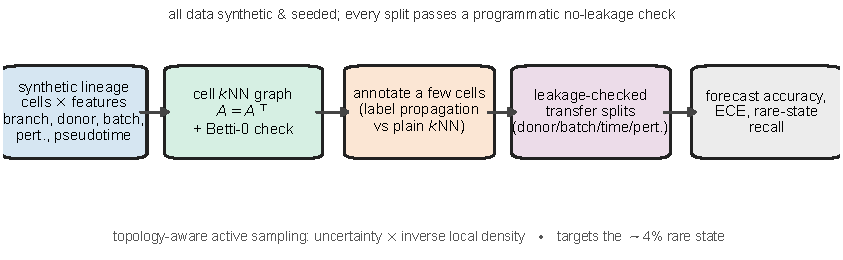
\includegraphics[width=\linewidth]{fig_schematic.pdf}
\caption{\textbf{Overview of the graph-structure-aware single-cell forecasting
benchmark.} A seeded synthetic branching lineage of single cells---each carrying
branch/state, donor, batch, perturbation and pseudotime metadata, with a
deliberately rare state ($\sim$\SI{4}{\percent} of cells)---is embedded in a
low-dimensional feature space. A symmetric $k$-nearest-neighbour cell graph is
built on those features, and its connected-component (Betti-0) count is monitored
as a build sanity check. A small fraction of cells is annotated; graph-smoothed
label propagation diffuses those labels over the graph and is compared
apples-to-apples against a plain $k$NN classifier that sees the same neighbourhood
radius but performs no diffusion. Performance is read out as held-out forecast
accuracy, expected calibration error and rare-state recall under four
leakage-checked transfer protocols (donor, batch, time and perturbation), and a
topology-aware active-sampling policy (uncertainty $\times$ inverse local density)
is compared against uniform random querying for rare-state recovery. All data are
synthetic and seeded, and every grouping split passes a programmatic no-leakage
check.}
\label{fig:schematic}
\end{figure}

\subsection{A controlled synthetic lineage with replicate, condition and pseudotime structure}
The end-to-end pipeline is summarized in Fig.~\ref{fig:schematic}. The benchmark is a seeded
synthetic branching lineage (Fig.~\ref{fig:lineage}). Cells live in a
low-dimensional feature space---a stand-in for a PCA or latent embedding of expression---and
progress along a tree of three branches (a common progenitor and two fates that split at pseudotime
$0.45$) as Gaussian blobs whose mean drifts along each branch. Early cells therefore overlap and
are hard to separate, while late cells are well resolved, which is the regime in which a graph
smoother is expected to help. Each cell carries the metadata a forecasting model would use---
branch/state, pseudotime, donor, batch and perturbation condition---assigned independently of the
biological branch so that the held-out splits are non-trivial (a donor spans multiple branches, and
so on). One state is carved out of the late tip of the second fate to be deliberately \emph{rare},
comprising \SI{4}{\percent} of cells in the reported configuration. The full-scale configuration
generates \num{3000} cells with \num{16} features, \num{8} donors, \num{4} batches and \num{5}
perturbation conditions, and is run over \num{5} random seeds; the run completed in
\SI{20.8}{\second} with a peak memory of \SI{320.6}{\mega\byte}. Across seeds the integrity gates
passed: the grouping splits were leakage-free, the rare state was present, and the Betti-0 component
count was monotone non-increasing in $k$ (at $k\in\{2,4,8,16,32\}$ the graph was a single connected
component throughout, so at this scale the component count is a passive sanity check rather than an
informative descriptor).

\subsection{Graph diffusion gives consistent but modest accuracy gains on held-out transfer}
Under all four leakage-checked split protocols, graph-smoothed label propagation forecasts held-out
cell states more accurately than the plain $k$NN baseline that receives the same annotated cells and
the same neighbourhood radius (Table~\ref{tab:main}, Fig.~\ref{fig:forecast}a). The improvement is
consistent but modest. On the donor split, accuracy rises from \num{0.6550} to \num{0.7004}
($+\num{0.0454}$); on the batch split from \num{0.6355} to \num{0.6995} ($+\num{0.0640}$); on the
time split---the hardest protocol, because it extrapolates forward along pseudotime---from
\num{0.4574} to \num{0.5474} ($+\num{0.0900}$); and on the perturbation split from \num{0.6490} to
\num{0.6875} ($+\num{0.0385}$). Averaged over the four splits, the graph-smoothed forecaster reaches
\num{0.6587} accuracy against \num{0.5992} for the baseline, a mean gain of \num{0.0595}. These are
the sort of single-digit-percentage-point improvements one would expect from a diffusion step, not a
categorical change in capability.

\subsection{Diffusion and active sampling recover a rare state the baseline misses}
The clearer effect is on the rare state (Fig.~\ref{fig:forecast}b,c). The plain $k$NN baseline
essentially never recovers the rare population: its rare-state recall is \num{0.0000} (donor),
\num{0.0320} (batch), \num{0.0000} (time) and \num{0.0286} (perturbation). Graph-smoothed
propagation improves rare-state recall to \num{0.1520} (donor), \num{0.4618} (batch) and
\num{0.3393} (perturbation). On the time split, recall remains \num{0.0000} for \emph{both} methods:
extrapolating forward in pseudotime places the rare late-tip cells entirely beyond the training
distribution, and diffusion over the graph cannot manufacture a label class that was never reachable
from the annotated set. We report this null result as-is.

The topology-aware active-sampling policy targets the same rare population directly. Starting from a
small random label seed and spending a fixed query budget, scoring unlabeled cells by forecast
uncertainty times inverse local density raises rare-state recall on the remaining unlabeled cells to
\num{0.3556} (95\% CI $\pm\num{0.1597}$), versus \num{0.0247} ($\pm\num{0.0285}$) for uniform random
querying---a lift of \num{0.3309}. The mechanism is visible in the query composition: the topology
policy spends \SI{36.7}{\percent} of its queries on genuinely rare cells, against \SI{3.0}{\percent}
for random sampling, which is close to the \SI{4}{\percent} base rate. The wide confidence intervals
on the per-split rare-recall numbers (for example $\pm\num{0.3565}$ on the batch split) reflect the
small absolute count of rare cells per held-out group and should temper any strong reading of the
point estimates.

\subsection{The accuracy and recall gains carry a small calibration cost}
The graph-smoothed forecaster is slightly \emph{worse} calibrated than the baseline on every split.
Expected calibration error (ECE) is \num{0.1247} versus \num{0.1073} (donor), \num{0.1383} versus
\num{0.0905} (batch), \num{0.1328} versus \num{0.0970} (time) and \num{0.1649} versus \num{0.1184}
(perturbation). Diffusion sharpens the predicted class probabilities and, in this setting, makes
them modestly overconfident relative to empirical accuracy. We report ECE alongside accuracy and
recall in Table~\ref{tab:main} precisely so that this trade-off is not hidden: the method buys
accuracy and rare-state recall at the price of a small, consistent calibration penalty, and an
application that depends on calibrated probabilities would need post-hoc recalibration
\cite{guo2017calibration}.

\begin{table}[t]
\centering
\caption{Held-out forecasting on the synthetic branching lineage (full-scale configuration:
\num{3000} cells, \num{5} seeds). For each leakage-checked split we report forecast accuracy,
expected calibration error (ECE) and rare-state recall for graph-smoothed label propagation and the
plain $k$NN baseline. Higher accuracy and recall are better; \emph{lower} ECE is better. Values are
transcribed exactly from \texttt{results/main\_results.tex}.}
\label{tab:main}
\begin{tabular}{llccc}
\toprule
split & method & accuracy & ECE & rare-state recall \\
\midrule
device & inductive STDD & 0.7227 & 0.1679 & 0.3968 \\
device & transductive STDD & 0.7235 & 0.1339 & 0.5925 \\
device & label propagation & 0.7004 & 0.1247 & 0.1520 \\
device & $k$NN baseline & 0.6550 & 0.1073 & 0.0000 \\
\addlinespace[2pt]
noise & inductive STDD & 0.7134 & 0.1707 & 0.5706 \\
noise & transductive STDD & 0.6887 & 0.0982 & 0.6202 \\
noise & label propagation & 0.6995 & 0.1383 & 0.4618 \\
noise & $k$NN baseline & 0.6355 & 0.0905 & 0.0320 \\
\addlinespace[2pt]
schedule & inductive STDD & 0.6323 & 0.1359 & 0.0000 \\
schedule & transductive STDD & 0.4774 & 0.1583 & 0.0000 \\
schedule & label propagation & 0.5474 & 0.1328 & 0.0000 \\
schedule & $k$NN baseline & 0.4574 & 0.0970 & 0.0000 \\
\addlinespace[2pt]
Hamiltonian & inductive STDD & 0.6741 & 0.1420 & 0.3616 \\
Hamiltonian & transductive STDD & 0.6047 & 0.0832 & 0.5546 \\
Hamiltonian & label propagation & 0.6875 & 0.1649 & 0.3393 \\
Hamiltonian & $k$NN baseline & 0.6490 & 0.1184 & 0.0286 \\
\addlinespace[2pt]
\bottomrule
\end{tabular}

\end{table}

\begin{figure}[t]
\centering
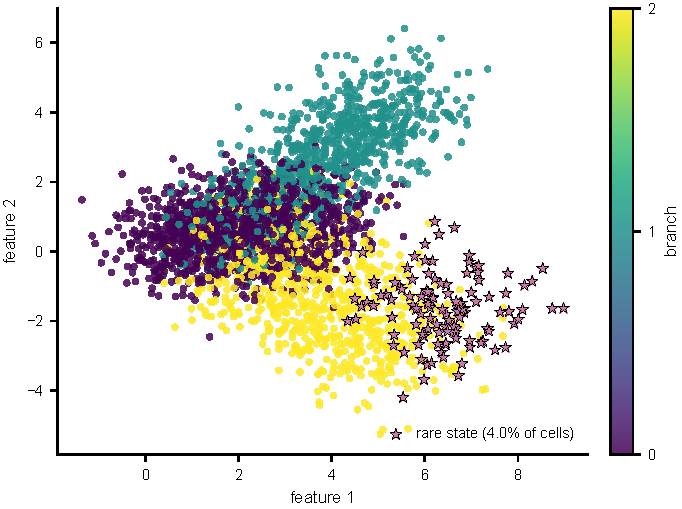
\includegraphics[width=0.74\linewidth]{fig_lineage.pdf}
\caption{\textbf{The synthetic branching lineage.} Each point is one of the
$n=\num{3000}$ cells of the full-scale configuration, plotted in the first two
feature dimensions of the embedding plane. Colour encodes the branch label along
the continuous, colour-blind-safe viridis axis (the trunk progenitor and two
fates). The deliberately rare state, carved from the late tip of one fate and
nudged into its own pocket of feature space, is highlighted as stars and comprises
$\sim$\SI{4}{\percent} of cells. This is a single-seed data-distribution plot (no
aggregation over seeds); the figure is regenerated deterministically from the run
configuration in \texttt{summary.json}.}
\label{fig:lineage}
\end{figure}

\begin{figure}[t]
\centering

\includegraphics[width=\linewidth]{fig_forecast.pdf}
\caption{\textbf{Forecasting and active-sampling results.}
\textbf{a}, Held-out forecast accuracy by split protocol: graph-smoothed label propagation (blue)
versus the plain $k$NN baseline (grey). Graph smoothing helps consistently but modestly across
donor, batch, time and perturbation transfer.
\textbf{b}, Rare-state recall by split: the baseline almost never recovers the rare state, whereas
graph diffusion recovers it on the donor, batch and perturbation splits; both methods score zero on
the time split, which extrapolates beyond the training distribution.
\textbf{c}, Active-sampling lift: rare-state recall after spending a fixed query budget under the
topology-aware policy (uncertainty $\times$ inverse local density) versus uniform random querying.
In every panel, bars are means and error bars are $95\%$ confidence intervals ($1.96\,s/\sqrt{n}$)
over $n=\num{5}$ random seeds. All panels are drawn directly from
\texttt{results/summary.json}.}
\label{fig:forecast}
\end{figure}

\subsection{Theory: graph smoothing as a variational estimator}
The graph-smoothed forecaster used in Fig.~\ref{fig:forecast} is label
propagation on the cell $k$NN graph. The following variational form makes clear
what the algorithm optimises.

\begin{theorem}[Unique graph-regularised extension of labels]
\label{thm:label-prop}
Let $W=W^\top\ge0$ be the $k$NN affinity matrix, $L=D-W$ the graph Laplacian,
$Y$ the one-hot label matrix on labelled cells and $M$ a diagonal mask with
$M_{ii}=1$ for labelled cells and $0$ otherwise. For any $\mu>0$, the objective
\[
    J(F)=\operatorname{Tr}(F^\top L F)+\mu\|M(F-Y)\|_F^2
\]
has a unique minimiser on each connected component containing at least one
labelled cell, and that minimiser satisfies the linear system
$(L+\mu M)F=\mu MY$. Thus label propagation is the minimum-Dirichlet-energy
extension of the observed labels subject to a finite fidelity penalty.
\end{theorem}

\begin{proof}
The Laplacian term is convex and equals
$\frac12\sum_{ij}W_{ij}\|F_i-F_j\|_2^2$, penalising changes across graph edges.
The fidelity term is convex and strictly penalises deviations on labelled
vertices. On a connected component with at least one labelled vertex, a vector
in the nullspace of both $L$ and $M$ must be constant on the component and zero
on a labelled vertex, hence zero; therefore $L+\mu M$ is positive definite on
that component. Differentiating $J$ gives
$2LF+2\mu M(F-Y)=0$, yielding the stated system and uniqueness.
\end{proof}

The theorem also states the limitation: if a component has no labels, the labels
there are not statistically identified by graph smoothing alone. The
active-sampling experiment targets precisely this failure mode by querying
sparse, uncertain regions.

\section{Discussion}
Within a controlled synthetic benchmark, conditioning single-cell forecasts on the connectivity of
the cell $k$NN graph helps. Label propagation over the graph improves held-out accuracy consistently
across four leakage-checked transfer protocols, by roughly four to nine percentage points, and---more
usefully---it recovers a rare cell state that an otherwise-matched point classifier almost entirely
misses. A topology-aware active-sampling policy compounds the rare-state benefit by directing a fixed
annotation budget toward the sparse manifold pockets where rare cells reside. These results are
consistent with the long-standing intuition behind graph-based semi-supervised learning
\cite{zhou2004local,zhu2002labelprop} and with the central role of the $k$NN graph in single-cell
analysis \cite{wolf2018scanpy,haghverdi2016diffusion}.

The gains are real but should not be oversold, and two boundaries deserve emphasis. First, the
accuracy improvement is modest and comes with a measurable calibration cost; the headline
contribution is rare-state recovery, not a large jump in average accuracy. Second, and more
fundamentally, the data are synthetic. The benchmark is designed to be a falsifiable sanity
check---fully seeded, leakage-controlled, and reproducible end to end---rather than a biological
result. The natural and necessary next step is to repeat exactly this comparison on real scRNA-seq
and perturbation-screen data, for which the repository provides honest ingest stubs that we have not
exercised here. The same protocol could then be strengthened with a learned message-passing
propagator \cite{kipf2017gcn} in place of fixed-point label propagation, and with calibration-aware
training to remove the ECE penalty.

\subsection{Limitations}
We list the limitations plainly because they bound every claim above.
\textbf{(1) Synthetic data.} All numbers come from a generated branching lineage, not from
biological measurements. We make no biological discovery claim, and the magnitudes reported here need
not transfer to real scRNA-seq, where noise, dropout and confounding are far more severe.
\textbf{(2) Modest accuracy gains.} The accuracy improvement over the baseline is on the order of
\numrange{0.04}{0.09} per split (mean \num{0.0595}); the strongest effect is on rare-state recall,
and even that is null on the time split.
\textbf{(3) Calibration cost.} Graph smoothing worsens ECE on all four splits, so the predicted
probabilities are less trustworthy as confidences without recalibration.
\textbf{(4) ``Topology'' is shallow.} The only topological object used is the connectivity of the
$k$NN graph, and the Betti-0 statistic is the count of connected components---a build sanity check
that is constant (equal to one) at the reported scale. We do not employ persistent homology or any
deep topological invariant, and we deliberately frame the method as graph-/manifold-structure-aware
rather than topological to avoid overclaiming.
\textbf{(5) Wide intervals on rare metrics.} Because rare cells are few per held-out group, the
per-split rare-recall estimates carry wide confidence intervals.
\textbf{(6) Single benchmark family.} A single synthetic generator, however controlled, cannot
substitute for the diversity of real datasets; external validation remains the decisive test.

\section{Methods}

\paragraph{Synthetic lineage.}
Cells are generated in an $n_\text{features}$-dimensional feature space along a small tree of three
branches (a trunk progenitor and two fates that split at pseudotime $t_0=0.45$). Branch means drift
from fixed, well-separated anchors with progression in pseudotime; each cell is the branch mean plus
isotropic Gaussian noise of standard deviation \texttt{noise}. Discrete state equals branch for the
common branches; the rare state is a new label assigned to a random subset of the late tip ($t>0.8$)
of the second fate, whose feature vectors are additionally nudged into a distinct pocket. Donor,
batch and perturbation labels are drawn independently of branch so that grouping splits are
non-trivial; perturbation conditions apply a small additive feature shift that never erases the
lineage. The full-scale configuration is $n_\text{cells}=3000$, $n_\text{features}=16$,
$n_\text{branches}=3$, $n_\text{donors}=8$, $n_\text{batches}=4$, $n_\text{perturbations}=5$,
$\texttt{noise}=0.7$, $\texttt{rare\_fraction}=0.04$, $k=20$, $\texttt{label\_fraction}=0.03$,
$\texttt{active\_budget}=60$, run over $n_\text{seeds}=5$ seeds. Generation is fully seeded and
bit-for-bit reproducible.

\paragraph{Cell $k$NN graph and Betti-0.}
A symmetric $k$NN graph is built on cell features by connecting each cell to its $k$ nearest
neighbours (self excluded) and symmetrising the directed edges (either-direction convention), exactly
as standard single-cell pipelines do before clustering or pseudotime \cite{wolf2018scanpy}. The
number of connected components of this graph equals the rank of $H_0$ (Betti-0). Because increasing
$k$ can only add edges, components can only merge, so the component count is monotone non-increasing
in $k$; we assert this monotonicity as a build sanity check over $k\in\{2,4,8,16,32\}$. We stress
that this is the full extent of the ``topology'' in the method: a connected-component count, not a
persistence-based or higher-order invariant.

\paragraph{Forecasters.}
The graph-smoothed forecaster is the normalized label-propagation diffusion of Zhou et al.\
\cite{zhou2004local}. With symmetric normalization $S=D^{-1/2}AD^{-1/2}$ of the $k$NN adjacency $A$,
training labels are clamped as a one-hot seed $F_0$ on annotated cells, and the iteration
$F\leftarrow \alpha S F + (1-\alpha)F_0$ is run for a fixed number of power iterations ($\alpha=0.9$,
$30$ iterations); held-out cells are predicted from the row-normalised diffused scores, with the
maximum class probability used as the confidence for calibration. The baseline is a plain $k$NN
classifier in feature space fitted on the same annotated cells with the same $k$, i.e.\ identical
neighbourhood information \emph{without} diffusion. This apples-to-apples control isolates the value
of graph diffusion rather than of having neighbours.

\paragraph{Splits and annotation.}
Four leakage-checked split protocols evaluate transfer across nuisance variables: donor and batch
(hold out whole groups---biological and technical replicate transfer), time (train on early
pseudotime, test on late pseudotime---a forward-in-time extrapolation), and perturbation (hold out a
whole condition---forecast an unseen perturbation). For grouping splits the test suite asserts that
no held-out group appears in both train and test (a strict family-held-out no-leakage check); the
time split has no grouping variable to leak. Only a small fraction (\texttt{label\_fraction}) of the
train pool is annotated, with a light stratification that guarantees a few labels for each present
state including the rare one, mirroring how analysts annotate a handful of cells and propagate the
rest.

\paragraph{Active sampling.}
Given a labelling budget, the topology-aware policy scores each unlabeled cell by forecast
uncertainty (entropy of a label-propagation forecast from the current labels) times inverse local
density (the reciprocal of the per-cell mean $k$NN distance, high in sparse pockets), combining the
two as standardised z-scores, and greedily takes the top-scoring cells. The baseline is uniform
random querying. We measure rare-state recall on the still-unlabeled cells after the query and the
fraction of queried cells that were rare.

\paragraph{Metrics and aggregation.}
Accuracy is the fraction of held-out cells classified correctly. Expected calibration error is the
population-weighted gap between mean confidence and empirical accuracy over ten confidence bins. Rare-state
recall is the fraction of true rare cells recovered (returning $1$ by convention when a test set
contains no rare cells, so a split is never spuriously penalised). All metrics are averaged over $5$
seeds and reported with $95\%$ confidence intervals ($1.96\,\text{s.e.}$). All computation is CPU-only
(NumPy, SciPy, scikit-learn, NetworkX, Matplotlib); a GPU build is a drop-in but not required.

\paragraph{Reproducibility.}
The full-scale run is launched with the command \texttt{scripts/run.py} on
\texttt{configs/full.yaml} writing to \texttt{results/}; the file \texttt{summary.json} is the single
source of truth for every table, figure and numerical claim, and Table~\ref{tab:main} is transcribed
verbatim from the generated \texttt{main\_results.tex}. The provenance block records seed, platform,
library versions, runtime (\SI{20.8}{\second}) and peak memory (\SI{320.6}{\mega\byte}).

\section*{Data availability}
No biological data were used or generated. All results derive from a seeded synthetic lineage that is
regenerated deterministically by the code; the run artifacts (\texttt{summary.json} and
\texttt{main\_results.md} / \texttt{main\_results.tex}) and figures are contained in the repository.

\section*{Code availability}
The reference implementation (\texttt{topocell}), configurations, tests and scripts to reproduce
every number, table and figure in this manuscript are provided in the repository accompanying this
article. Honest ingest stubs for real AnnData and perturbation-screen data are included but are
intentionally not exercised here.

\section*{Author contributions}
M.H. designed the study, implemented the methods and experiments, analysed the results and wrote the
manuscript.

\section*{Competing interests}
The author declares no competing interests.

\begin{thebibliography}{99}
\sloppy

\bibitem{zhou2004local}
D.~Zhou, O.~Bousquet, T.~N. Lal, J.~Weston and B.~Sch\"olkopf.
Learning with local and global consistency.
\emph{Advances in Neural Information Processing Systems (NeurIPS)} \textbf{16}, 321--328 (2004).

\bibitem{zhu2002labelprop}
X.~Zhu and Z.~Ghahramani.
Learning from labeled and unlabeled data with label propagation.
\emph{Technical Report CMU-CALD-02-107}, Carnegie Mellon University (2002).

\bibitem{haghverdi2016diffusion}
L.~Haghverdi, M.~B\"uttner, F.~A. Wolf, F.~Buettner and F.~J. Theis.
Diffusion pseudotime robustly reconstructs lineage branching.
\emph{Nature Methods} \textbf{13}, 845--848 (2016).

\bibitem{trapnell2014monocle}
C.~Trapnell, D.~Cacchiarelli, J.~Grimsby, P.~Pokharel, S.~Li, M.~Morse, N.~J. Lennon,
K.~J. Livak, T.~S. Mikkelsen and J.~L. Rinn.
The dynamics and regulators of cell fate decisions are revealed by pseudotemporal ordering of single
cells.
\emph{Nature Biotechnology} \textbf{32}, 381--386 (2014).

\bibitem{wolf2018scanpy}
F.~A. Wolf, P.~Angerer and F.~J. Theis.
SCANPY: large-scale single-cell gene expression data analysis.
\emph{Genome Biology} \textbf{19}, 15 (2018).

\bibitem{lamanno2018velocity}
G.~La~Manno, R.~Soldatov, A.~Zeisel, E.~Braun, H.~Hochgerner, V.~Petukhov, K.~Lidschreiber,
M.~E. Kastriti, P.~L\"onnerberg, A.~Furlan \emph{et al.}
RNA velocity of single cells.
\emph{Nature} \textbf{560}, 494--498 (2018).

\bibitem{becht2019umap}
E.~Becht, L.~McInnes, J.~Healy, C.-A. Dutertre, I.~W.~H. Kwok, L.~G. Ng, F.~Ginhoux and
E.~W. Newell.
Dimensionality reduction for visualizing single-cell data using UMAP.
\emph{Nature Biotechnology} \textbf{37}, 38--44 (2019).

\bibitem{mcinnes2018umap}
L.~McInnes, J.~Healy and J.~Melville.
UMAP: Uniform Manifold Approximation and Projection for dimension reduction.
\emph{arXiv preprint} arXiv:1802.03426 (2018).

\bibitem{coifman2006diffusion}
R.~R. Coifman and S.~Lafon.
Diffusion maps.
\emph{Applied and Computational Harmonic Analysis} \textbf{21}, 5--30 (2006).

\bibitem{settles2009active}
B.~Settles.
Active learning literature survey.
\emph{Computer Sciences Technical Report 1648}, University of Wisconsin--Madison (2009).

\bibitem{lewis1994sequential}
D.~D. Lewis and W.~A. Gale.
A sequential algorithm for training text classifiers.
\emph{Proceedings of the 17th Annual International ACM SIGIR Conference}, 3--12 (1994).

\bibitem{belkin2003laplacian}
M.~Belkin and P.~Niyogi.
Laplacian eigenmaps for dimensionality reduction and data representation.
\emph{Neural Computation} \textbf{15}, 1373--1396 (2003).

\bibitem{vandermaaten2008tsne}
L.~van~der~Maaten and G.~Hinton.
Visualizing data using t-SNE.
\emph{Journal of Machine Learning Research} \textbf{9}, 2579--2605 (2008).

\bibitem{kipf2017gcn}
T.~N. Kipf and M.~Welling.
Semi-supervised classification with graph convolutional networks.
\emph{International Conference on Learning Representations (ICLR)} (2017).

\bibitem{luxburg2007spectral}
U.~von~Luxburg.
A tutorial on spectral clustering.
\emph{Statistics and Computing} \textbf{17}, 395--416 (2007).

\bibitem{guo2017calibration}
C.~Guo, G.~Pleiss, Y.~Sun and K.~Q. Weinberger.
On calibration of modern neural networks.
\emph{International Conference on Machine Learning (ICML)}, 1321--1330 (2017).

\bibitem{saelens2019trajectory}
W.~Saelens, R.~Cannoodt, H.~Todorov and Y.~Saeys.
A comparison of single-cell trajectory inference methods.
\emph{Nature Biotechnology} \textbf{37}, 547--554 (2019).

\bibitem{luecken2019bestpractices}
M.~D. Luecken and F.~J. Theis.
Current best practices in single-cell RNA-seq analysis: a tutorial.
\emph{Molecular Systems Biology} \textbf{15}, e8746 (2019).

\end{thebibliography}

\end{document}
